\documentclass[a4paper,10pt,twoside]{article}
\usepackage[polish]{babel}
\usepackage[utf8]{inputenc}
\usepackage[T1]{fontenc}
\usepackage{indentfirst}
\usepackage[top=2.5cm, bottom=2.5cm, left=2.5cm, right=2.5cm]{geometry}
\usepackage{graphicx}
\usepackage{amsmath}
\usepackage{booktabs}

\begin{document}

\newcommand{\unit}[1]{\thinspace \mathrm{#1}}

\begin{center}
\bgroup
\def\arraystretch{1.5}
\begin{tabular}{|c|c|c|c|c|c|}
	\hline
	EAIiIB & \multicolumn{2}{|c|}{Piotr Morawiecki, Tymoteusz Paszun} & Rok II & {Grupa 3a} & {Zespół 6} \\
	\hline
	\multicolumn{3}{|c|}{\begin{tabular}{c}Temat: Moduł Younga \end{tabular}} & 
	\multicolumn{3}{|c|}{\begin{tabular}{c}Numer ćwiczenia: 11 \end{tabular}} \\
	\hline
	\begin{tabular}{@{}c@{}}Data wykonania:\\8.11.2017r.\end{tabular} & \begin{tabular}{@{}c@{}}Data oddania:\\15.11.2017r.\end{tabular} & 
	\begin{tabular}{c}Zwrot do poprawki:\\\phantom{data} \end{tabular} & \begin{tabular}{c}Data oddania:\\\phantom{data}\end{tabular} &
	\begin{tabular}{@{}c@{}}Data zaliczenia:\\\phantom{data}\end{tabular} & \begin{tabular}{c}Ocena:\\\phantom{ocena}\end{tabular} \\[4ex]
	\hline
\end{tabular}
\egroup
\end{center}


\section{Cel ćwiczenia}

Celem ćwiczenia jest wyznaczenie modułu Younga metodą statyczną przy pomocy pomiaru wydłużenia drutu obciążonego stałą siłą. 

\section{Wstęp teoretyczny}


$$ \Delta l = \frac{Fl}{ES} $$

$$ \sigma = E \varepsilon $$

\section{Opis doświadczenia}

\begin{figure}[!htp]
\centerline{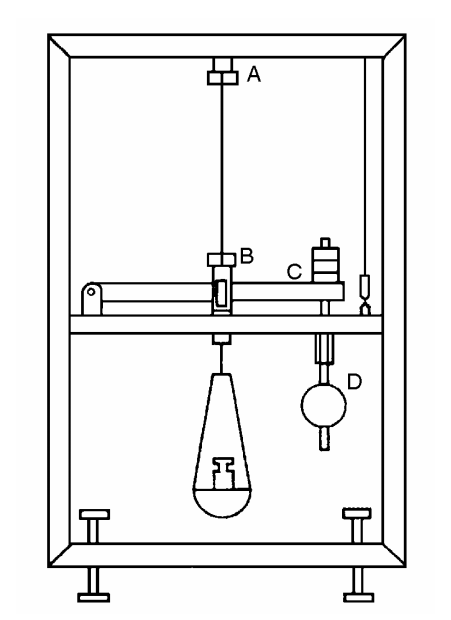
\includegraphics[scale=0.35]{przyrzad.png}}
\caption{Przyrząd pomiarowy}
\label{fig:tl}
\end{figure}

\section{Wyniki pomiarów}

\begin{table}[!htbp]
\caption{Pomiary dla drutu wykonanego ze stali}
\centering
\def\arraystretch{1.4}
\begin{tabular}{@{}rcccc@{}}
\\
\toprule
\begin{tabular}{@{}c@{}}Masa odważników $[\unit{kg}]$\end{tabular} &
\begin{tabular}{@{}c@{}}Siła $F \unit{[N]}$\end{tabular} &
\begin{tabular}{@{}c@{}}Wskazanie czujnika przy \\ dodawaniu obciążenia\end{tabular} &
\begin{tabular}{@{}c@{}}Wskazanie czujnika przy 
\\ odejmowaniu obciążenia\end{tabular} &
\begin{tabular}{@{}c@{}}$\Delta l \unit{[mm]}$\end{tabular}\\
\midrule
0,957  &   9,38817  &  0,290  &  0,38  &  0,16750 \\
1,968  &  19,30608  &  0,780  &  0,83  &  0,40250 \\
2,956  &  28,99836  &  1,110  &  1,17  &  0,57000 \\
3,951  &  38,75931  &  1,425  &  1,48  &  0,72625 \\
4,918  &  48,24558  &  1,780  &  1,78  &  0,89000 \\
5,946  &  58,33026  &  2,070  &  2,07  &  1,03500 \\
6,928  &  67,96368  &  2,320  &  2,38  &  1,17500 \\
7,961  &  78,09741  &  2,630  &  2,65  &  1,32000 \\
8,989  &  88,18209  &  2,915  &  2,92  &  1,45875 \\
9,972  &  97,82532  &  3,230  &        &  1,61500 \\
\bottomrule
\end{tabular}
\end{table}

\begin{table}[!htbp]
\caption{Pomiary dla drutu wykonanego z mosiądzu}
\centering
\def\arraystretch{1.4}
\begin{tabular}{@{}rcccc@{}}
\\
\toprule
\begin{tabular}{@{}c@{}}Masa odważników $[\unit{kg}]$\end{tabular} &
\begin{tabular}{@{}c@{}}Siła $F \unit{[N]}$\end{tabular} &
\begin{tabular}{@{}c@{}}Wskazanie czujnika przy \\ dodawaniu obciążenia\end{tabular} &
\begin{tabular}{@{}c@{}}Wskazanie czujnika przy 
\\ odejmowaniu obciążenia\end{tabular} &
\begin{tabular}{@{}c@{}}$\Delta l \unit{[mm]}$\end{tabular}\\
\midrule
0,957  &   9,38817  &  0,42  &  0,43  &  0,2125  \\
1,968  &  19,30608  &  0,91  &  0,92  &  0,4575  \\
2,956  &  28,99836  &  1,31  &  1,33  &  0,6600  \\
3,951  &  38,75931  &  1,70  &  1,73  &  0,8575  \\
4,918  &  48,24558  &  2,06  &  2,08  &  1,0350  \\
5,946  &  58,33026  &  2,44  &        &  1,2200  \\
\bottomrule
\end{tabular}
\end{table}


\newpage

\section{Wykresy}

\begin{figure}[!htp]
\centerline{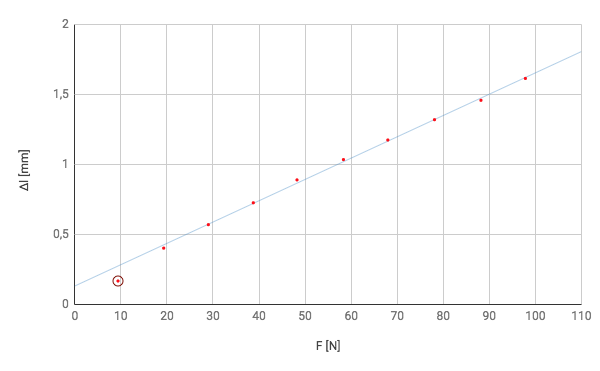
\includegraphics[scale=0.65]{steel_wire_first_point_marked.png}}
\caption{Wykres zależnosci wydłużenia drutu od przyłożonej siły dla stali}
\label{fig:tl}
\end{figure}

\begin{figure}[!htp]
\centerline{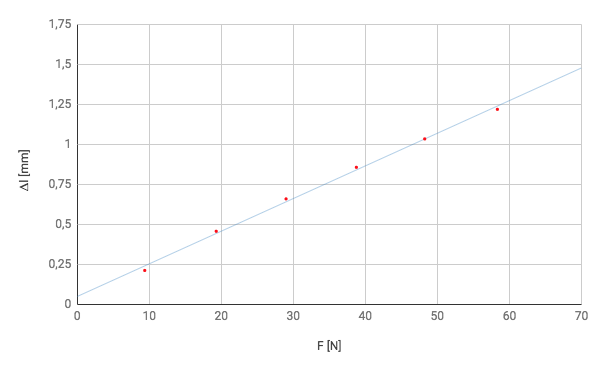
\includegraphics[scale=0.65]{brass_wire.png}}
\caption{Wykres zależnosci wydłużenia drutu od przyłożonej siły dla mosiądzu}
\label{fig:tl}
\end{figure}

\section{Opracowanie wyników}

\section{Wnioski}

\end{document}
